\begingroup
\setlength{\unitlength}{1bp}
\resizebox{.95\linewidth}{!}{\begin{picture}(984,1001)
\put(0,0){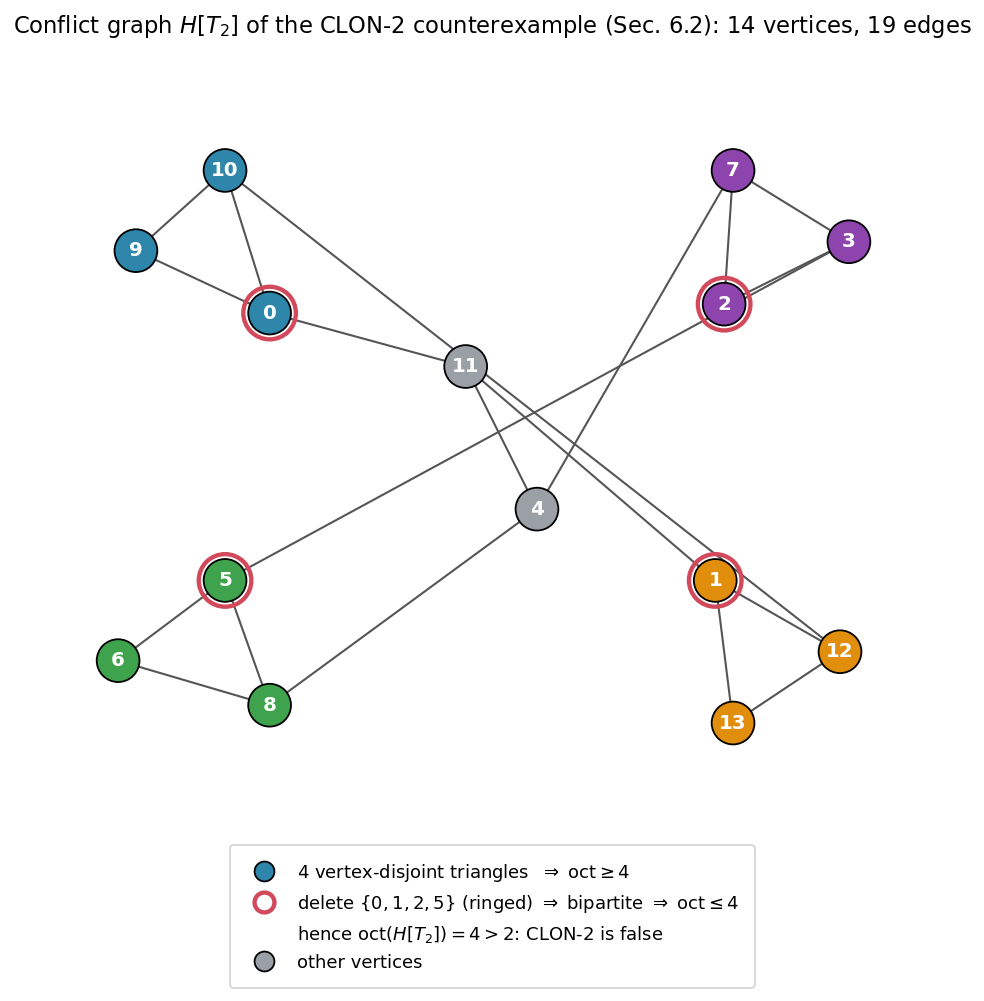
\includegraphics[width=984bp,height=1001bp]{figures/fig3_clon2_oct_en.png}}
\put(0,943){\color{white}\rule{984bp}{58bp}}
\put(492.0,972.0){\makebox(0,0){\raisebox{-.35\height}{\color{black}\fontsize{22}{24}\selectfont\sffamily Grafo \(H[T_2]\) del contraejemplo CLON-2 (\S9.2): 14 vértices, 19 aristas}}}
\put(288,112){\color{white}\rule{458bp}{39bp}}
\put(517.0,131.5){\makebox(0,0){\raisebox{-.35\height}{\color{black}\fontsize{18}{20}\selectfont\sffamily 4 triángulos disjuntos en vértices \(\Rightarrow\operatorname{oct}\ge4\)}}}
\put(288,82){\color{white}\rule{458bp}{30bp}}
\put(517.0,97.0){\makebox(0,0){\raisebox{-.35\height}{\color{black}\fontsize{17}{19}\selectfont\sffamily eliminar \(\{0,1,2,5\}\) (círculos) \(\Rightarrow\) bipartito \(\Rightarrow\operatorname{oct}\le4\)}}}
\put(288,50){\color{white}\rule{458bp}{32bp}}
\put(517.0,66.0){\makebox(0,0){\raisebox{-.35\height}{\color{black}\fontsize{18}{20}\selectfont\sffamily por tanto \(\operatorname{oct}(H[T_2])=4>2\): CLON-2 es falso}}}
\put(288,18){\color{white}\rule{458bp}{32bp}}
\put(517.0,34.0){\makebox(0,0){\raisebox{-.35\height}{\color{black}\fontsize{18}{20}\selectfont\sffamily otros vértices}}}
\end{picture}}
\endgroup
